\documentclass[a4paper,12pt]{report}


% Preambule.tex
% Packages de base
\usepackage[utf8]{inputenc}
\usepackage[T1]{fontenc}
\usepackage{pdfpages}
\usepackage[english]{babel} % Langue française
\usepackage{amsmath, amssymb} % Mathématiques
\usepackage{graphicx} % Insertion d'images
\usepackage{hyperref} % Hyperliens
\usepackage{geometry} % Mise en page
\usepackage{fancyhdr} % Pour personnaliser l'en-tête et le pied de page
\usepackage{float}
\usepackage{titlesec}
\usepackage{caption}


% Configurations spécifiques
\geometry{a4paper, margin=2.5cm} % Marges de la page
\setlength{\parskip}{\baselineskip} % Espacement entre les paragraphes
\setlength{\parindent}{0pt} % Pas d'indentation au début des paragraphes

\titleformat{\chapter}[hang]  % Utilisation du format 'hang' pour que tout soit sur la même ligne
  {\normalfont\huge\bfseries} % Style du titre (police normale, taille énorme, gras)
  {Chapter \thechapter\ \, :\ } % Format "Chapter" suivi du numéro du chapitre et des deux-points avec un espace après
  {0pt}                        % Pas d'espace supplémentaire
  {\huge}                       % Taille du texte du titre du chapitre


\usepackage{background}
\backgroundsetup{
scale=1,
angle=0,
opacity=1,
color=black,
contents={\begin{tikzpicture}[remember picture,overlay]
\node at ([xshift=-0.8in,yshift=0.8in] current page.south east) % Adjust the position of the logo.
{
\includegraphics[scale=0.8]{image/pattern.png}}; % logo goes here
\end{tikzpicture}}
}

\begin{document}
\raggedbottom
% Title page
\begin{titlepage}
    \centering

    
    \noindent 
    \begin{minipage}{0.5\textwidth}
        
\includegraphics[width=0.5\linewidth]{image/Logo_INSAToulouse-quadri.png} 
    \end{minipage}%
    \hfill 
    \begin{minipage}{0.5\textwidth}
        \flushright 
        
\includegraphics[width=0.5\linewidth]{image/logo_universite_toulouse.png}
    \end{minipage}


    \vspace*{2cm} 
    {\Huge\bfseries Portfolio \par}
    \vspace{1cm}
    {\huge Innovative Smart System \par}
    \vspace{2cm}
    {\Large \textbf{VASSEUR Cyril} \par}
    \vspace{2cm}

    \begin{figure}[H]
        \centering
        
\includegraphics[width=0.6\textwidth]{image/LOGO_ISS.png}
    \end{figure}
    
    \vfill
    {\Large \textbf{Institut National des Sciences Appliquées de Toulouse} \par}
    \vspace{1cm}
    {\large \today \par}
\end{titlepage}


\begin{abstract}

    This portfolio was prepared as part of the second year of a Master’s program in Innovative Smart Systems (ISS) at INSA Toulouse.
    Its purpose is to provide a comprehensive overview of my academic year, detailing the skills and knowledge I gained, along with my reflections on each course taken during the program.
    Within this portfolio, you’ll find summaries of each course, including insights on the topics covered and my personal assessments. 
    Additionally, it includes reports from practical sessions (laboratory work) and project-based exercises that allowed me to apply theoretical concepts in real-world contexts.

\end{abstract}


% Table of content
\renewcommand\contentsname{Table of contents}
\tableofcontents
\newpage

% Inclusion des chapter
\chapter{Introduction}

Dans le cadre de ma 5 ème Annéeà l'INSA Toulouse, j'ai eu l'occasion de me spécialisé dans le domaine de l'innovative smart system.
Dans la première partie vous retrouverez des informations sur ma scolarité, ainsi que mon CV qui vous informerons un peu mieux sur qui je suis.

\chapter{General Information}

\section{Presentation of MS Innovative Smart System}

The \textbf{Internet of Things (IoT)} is expected to grow rapidly in the coming years. Often described as the fourth industrial revolution, IoT is a promising field, with over 20 billion smart devices projected to be connected by 2020. However, achieving this scale will involve overcoming several challenges at multiple levels. 

The \textbf{Innovative Smart Systems Master’s Program} aims to prepare young engineers to understand and tackle these challenges by developing innovative solutions. IoT systems consist of multiple layers, each with its own focus:

\begin{itemize}
    \item Perceptual Layer
    \item Network Layer
    \item Support Layer
    \item Application Layer
\end{itemize}

Each of these layers has specific challenges, addressed by different training units in the program:

\begin{itemize}
\item Designing smart devices: \textit{Smart Devices Training Unit}
\item Connecting devices: \textit{Communication Training Unit}
\item Processing data within the network: \textit{Data Processing Training Unit}
\item Providing services for network interaction and data access: \textit{Middleware and Services Training Unit}
\end{itemize}

This master’s program addresses these challenges through a variety of courses, bringing together students from diverse fields, including Electronics, Telecommunications, Computer Science, and Physics. By combining these skills, students can collaborate to solve the complex problems involved in developing IoT networks and systems.

\section{Curriculum}

\subsection{Student Profile}

\textbf{Personal information :} \\
Surname: VASSEUR.  \\
First name: Cyril.  \\
email: vasseu@insa-toulouse.fr.  \\

\subsection{Curriculum Vitae}


\noindent
\begin{minipage}{\textwidth} 
    \centering
    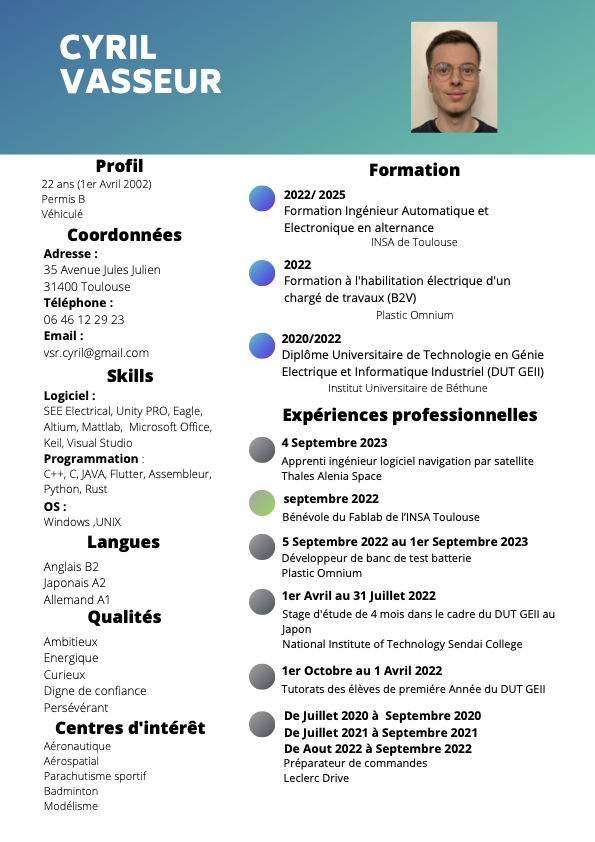
\includegraphics[width=0.8\textwidth]{image/CV_CYRIL VASSEUR.png}
    \label{fig:CV} 
\end{minipage}

\vspace{1em} 

\newpage
\subsection{Background}

Before entering INSA for my third year of higher education, I completed a two-year technical diploma (DUT) in Electrical Engineering and Industrial Computing at IUT of Béthune. 
I then pursued an engineering degree at INSA Toulouse, where I began a Master’s in Automation and Electronics through an apprenticeship program. 
My first year was spent with Plastic Omnium, where I worked on developing a test bench for heavy vehicle batteries used in trains and trucks. 
For my second year, I moved to Thales Alenia Space, drawn by my interest in the space sector, where I became a software apprentice specializing in satellite navigation.
After completing my Master’s, I continued at Thales Alenia Space to pursue my second Master’s in Innovative Smart Systems (ISS).



\subsection{Training units}

Below, you can find the overview of the various courses completed in the ISS program.

\begin{figure}[!ht]
    \centering
    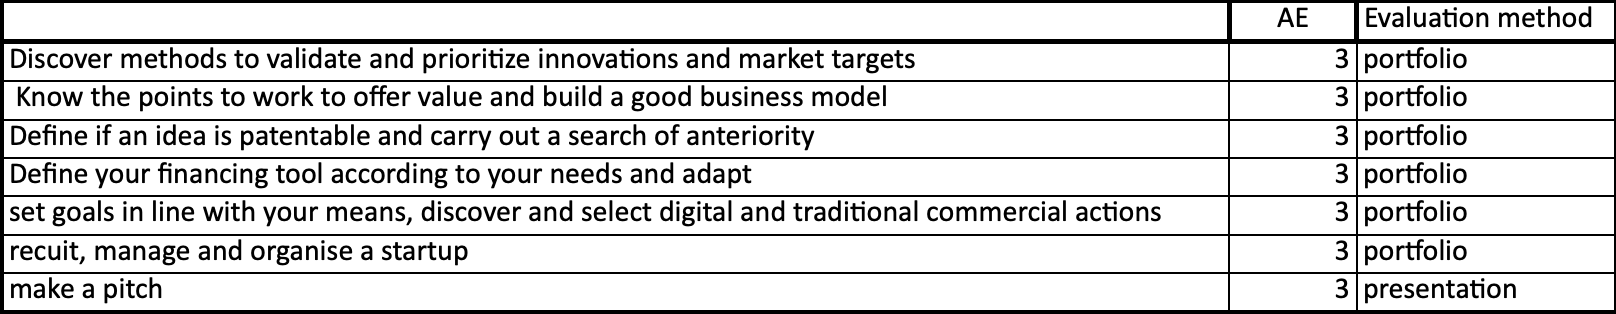
\includegraphics[width=0.8\textwidth]{image/Business startup.png}
    \caption{Business Startup Unit}
    \label{fig:Business Startup Unit}
\end{figure}
\begin{figure}[!ht]
    \centering
    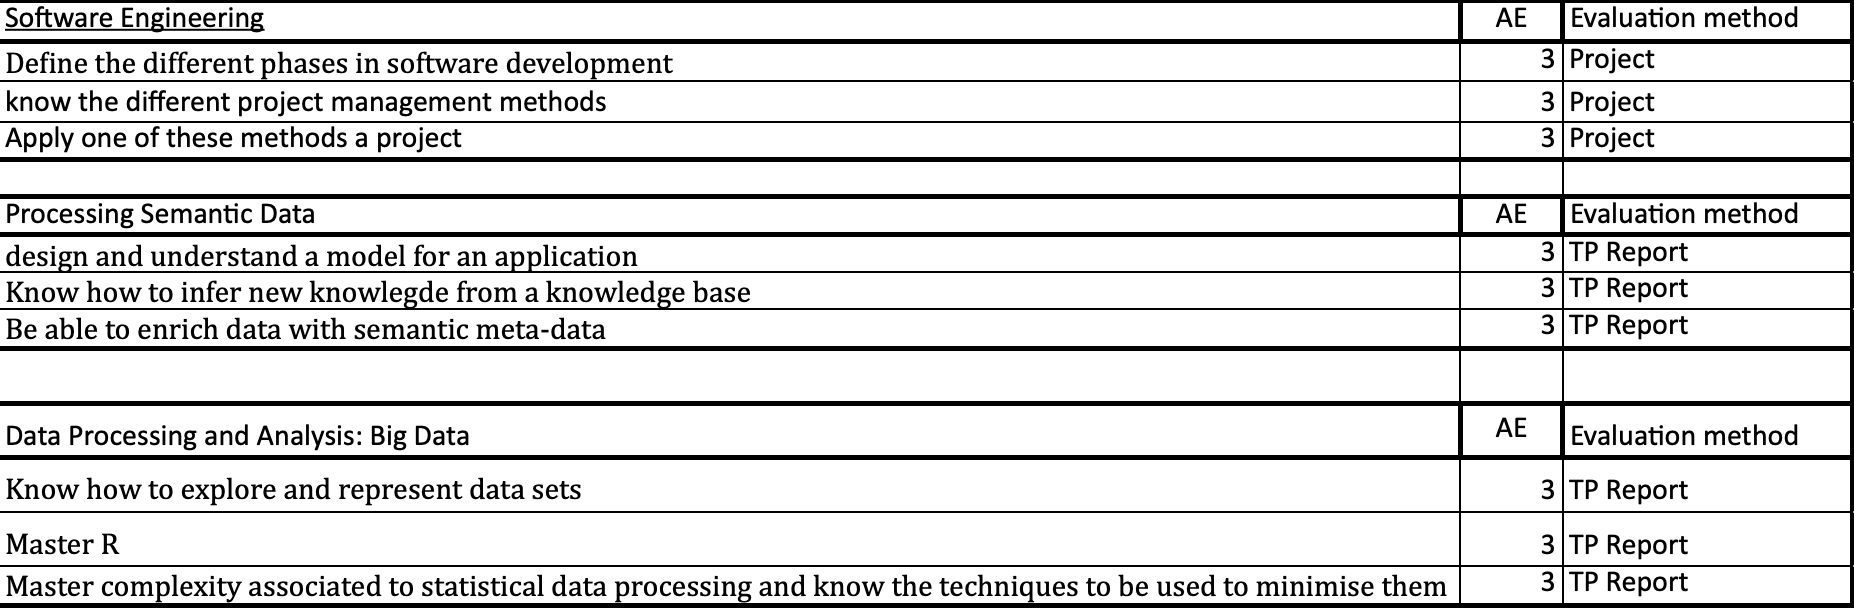
\includegraphics[width=0.8\textwidth]{image/Analysis and data processing, business applications.png}
    \caption{Analysis and data processing, business applications Unit}
    \label{fig:Analysis and data processing, business applications}
\end{figure}
\begin{figure}[!ht]
    \centering
    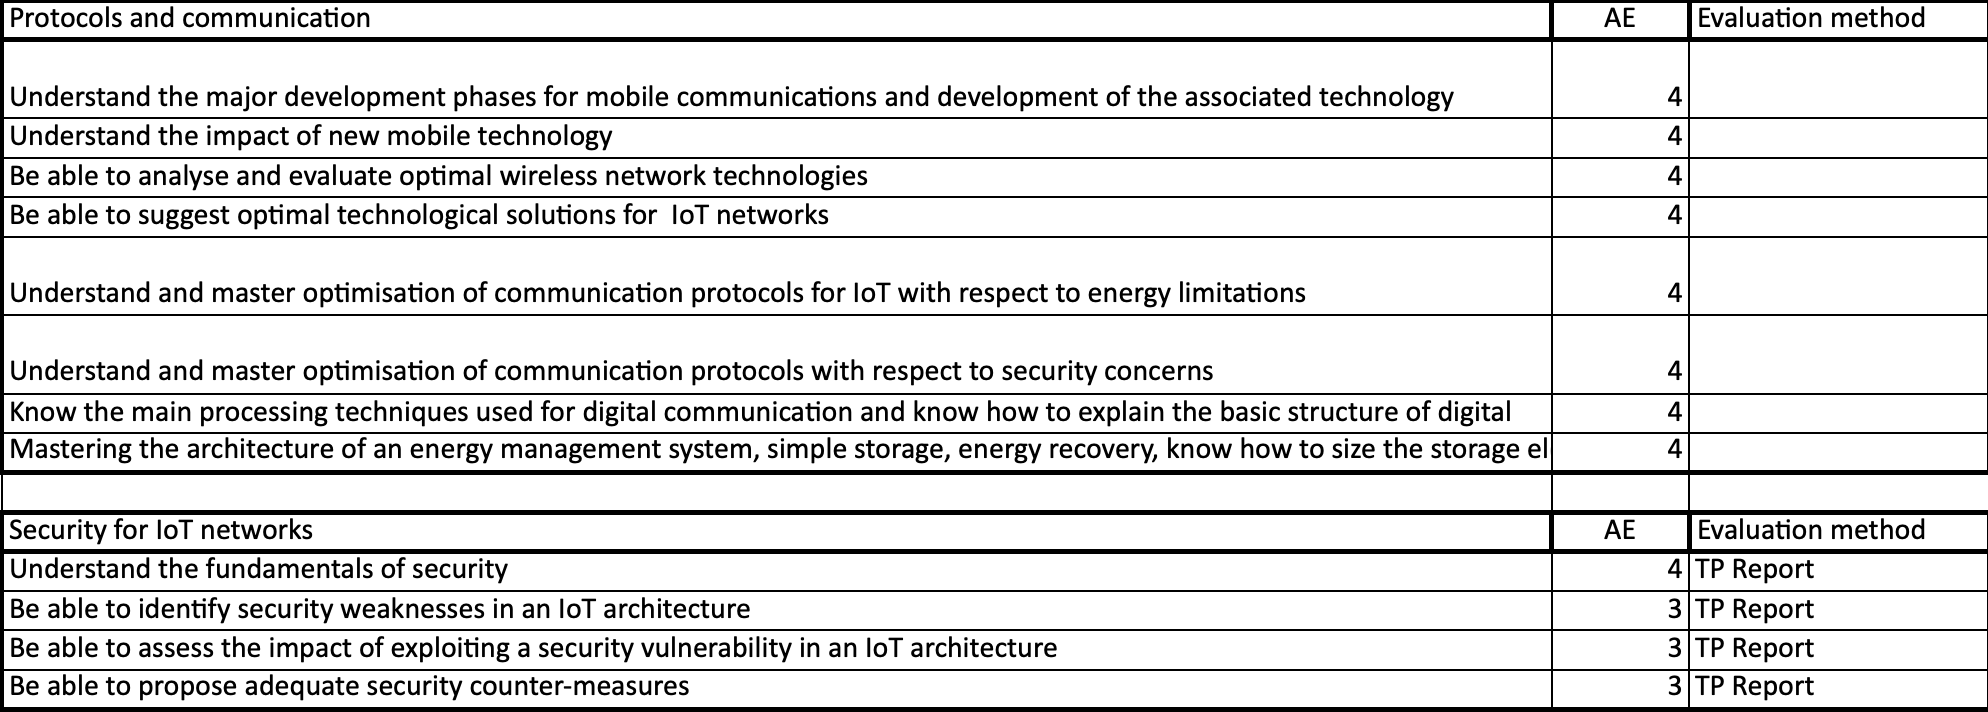
\includegraphics[width=0.8\textwidth]{image/Communication.png}
    \caption{Communication Unit}
    \label{fig:Communication}
\end{figure}
\begin{figure}[!ht]
    \centering
    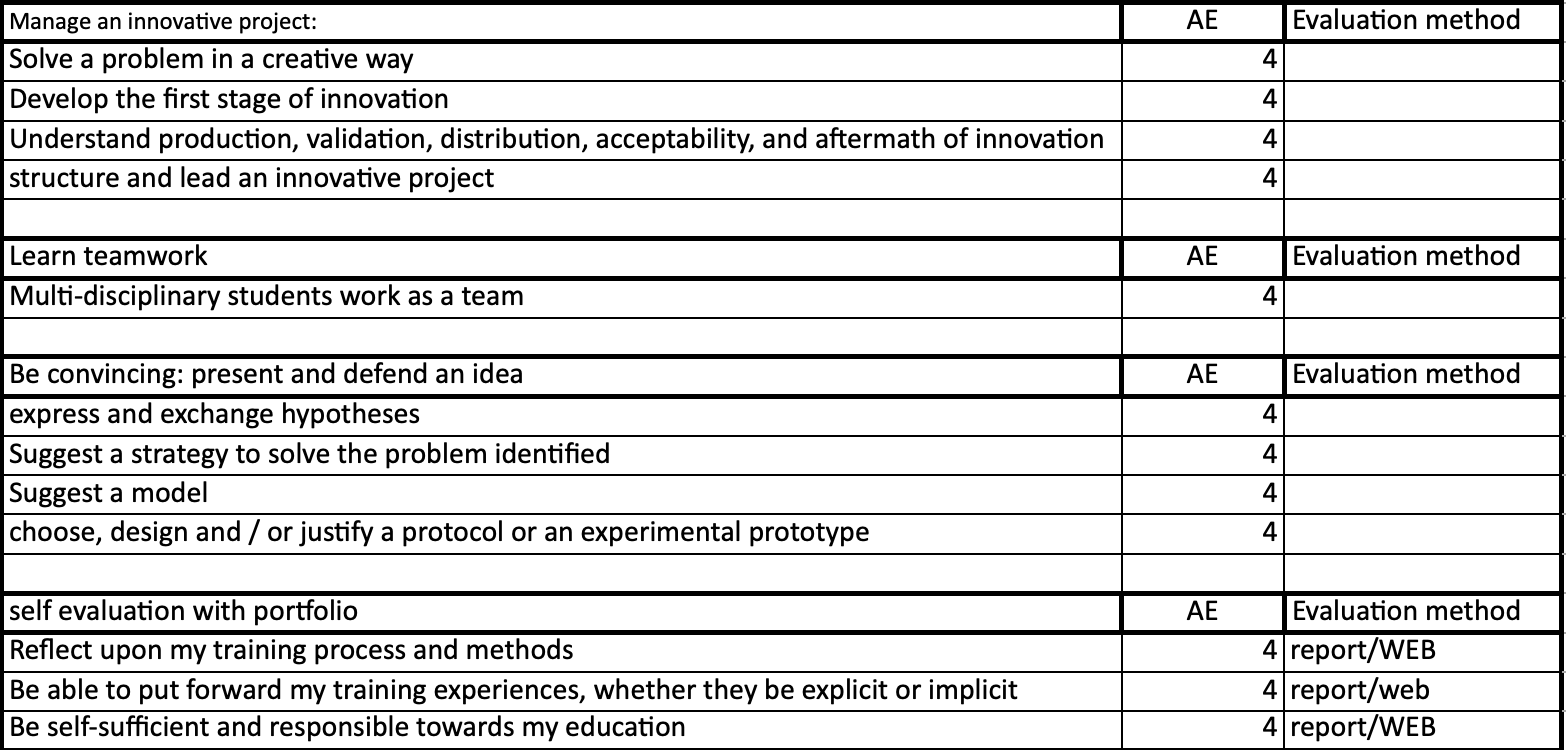
\includegraphics[width=0.8\textwidth]{image/Innovation and humanity.png}
    \caption{Innovation and humanity Unit}
    \label{fig:Innovation and humanity}
\end{figure}
\begin{figure}[!ht]
    \centering
    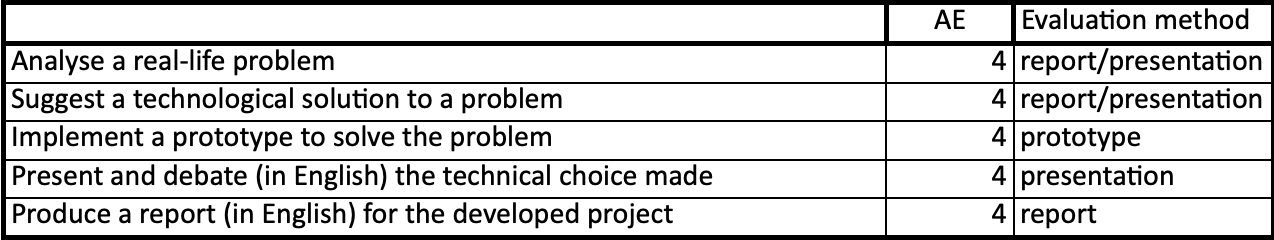
\includegraphics[width=0.8\textwidth]{image/Innovativ project.png}
    \caption{Innovative project Unit}
    \label{fig:Innovativ project}
\end{figure}
\begin{figure}[!ht]
    \centering
    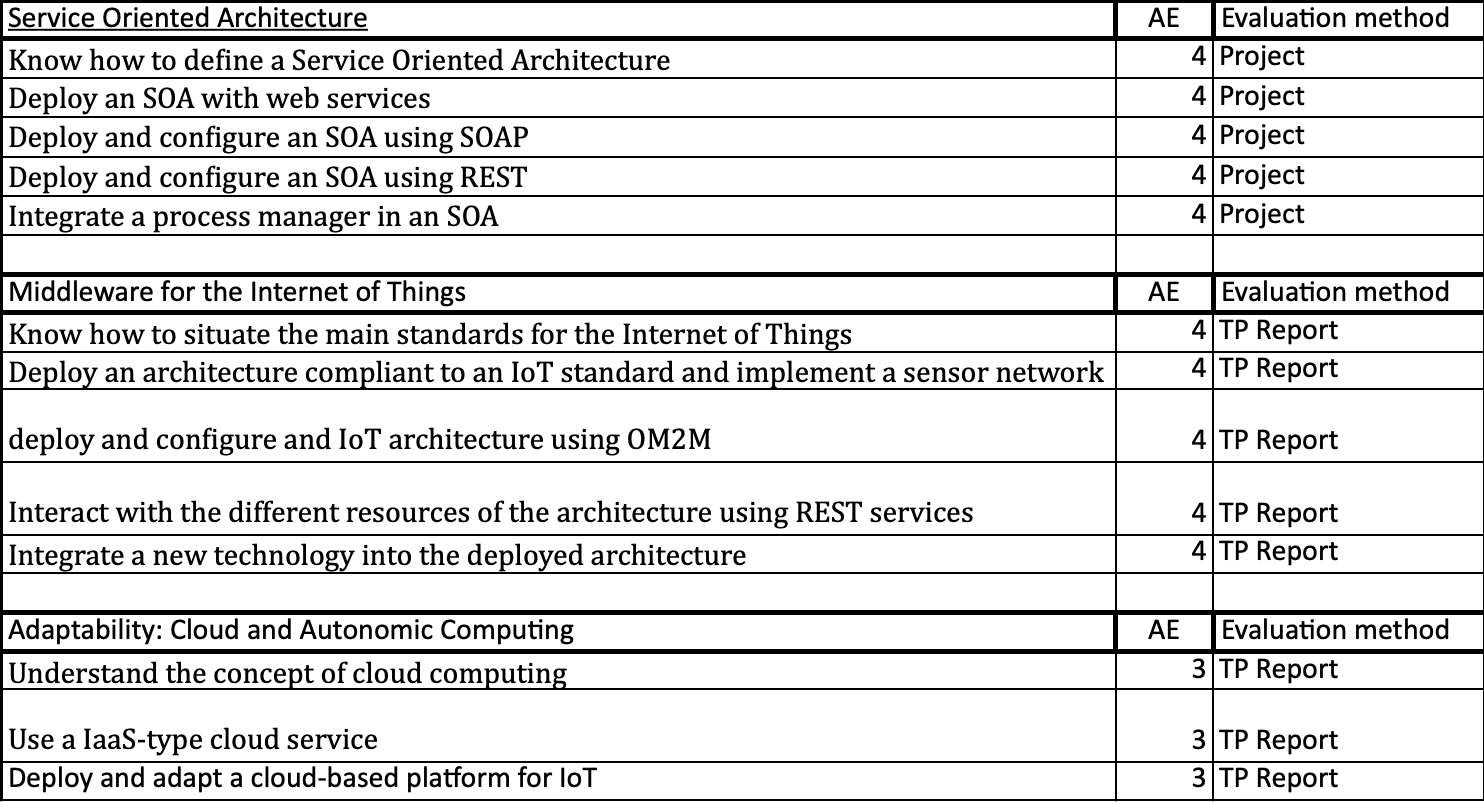
\includegraphics[width=0.8\textwidth]{image/Middleware and Service.png}
    \caption{Middleware and Service Unit}
    \label{fig:Middleware and Service}
\end{figure}
\begin{figure}[!ht]
    \centering
    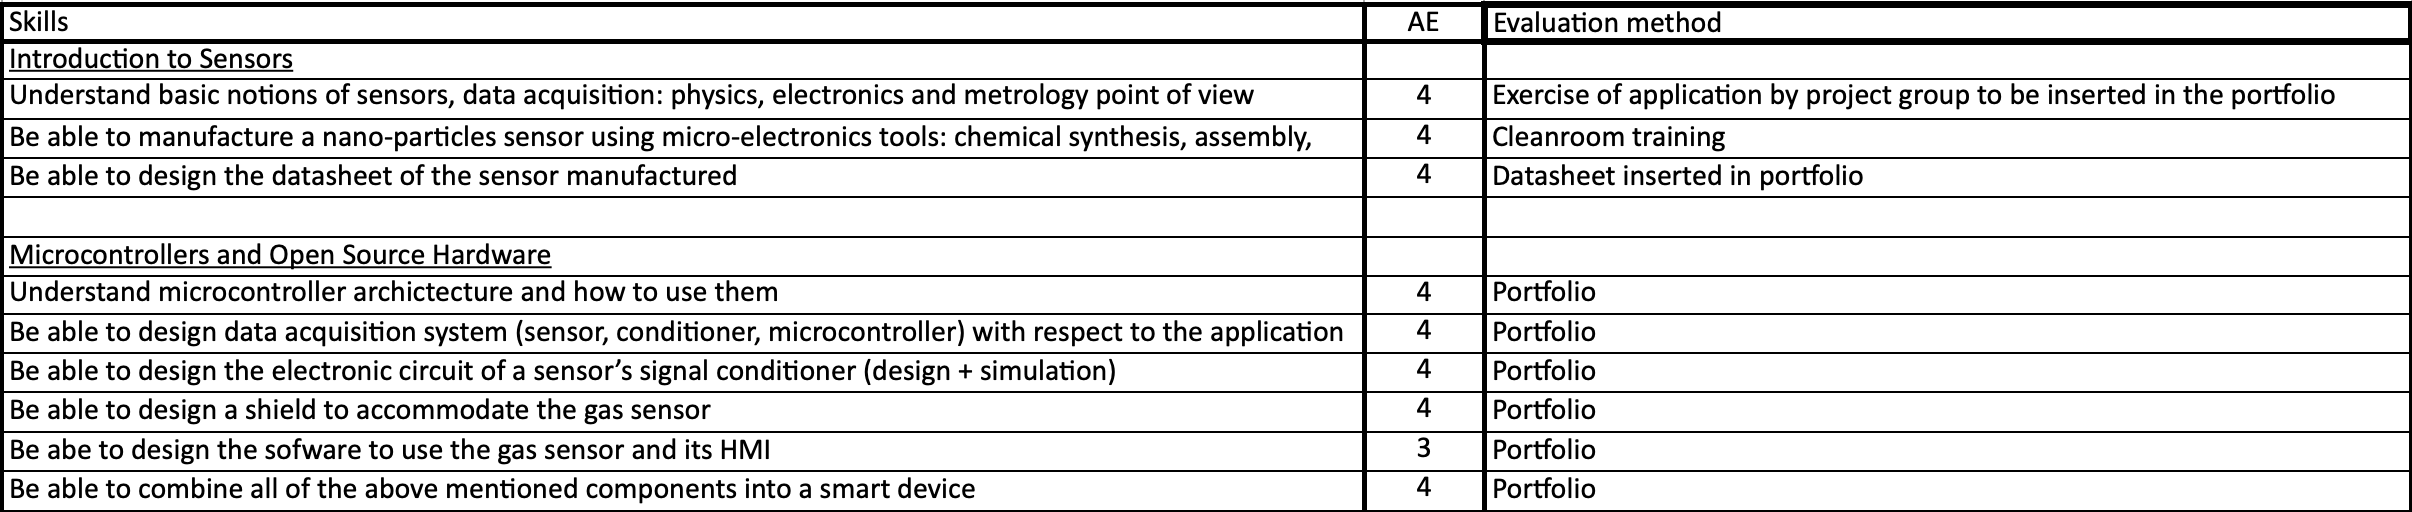
\includegraphics[width=0.8\textwidth]{image/Smart devices.png}
    \caption{Smart devices Unit}
    \label{fig:Smart devices}
\end{figure}
\newpage
\begin{figure}[H]
    \centering
    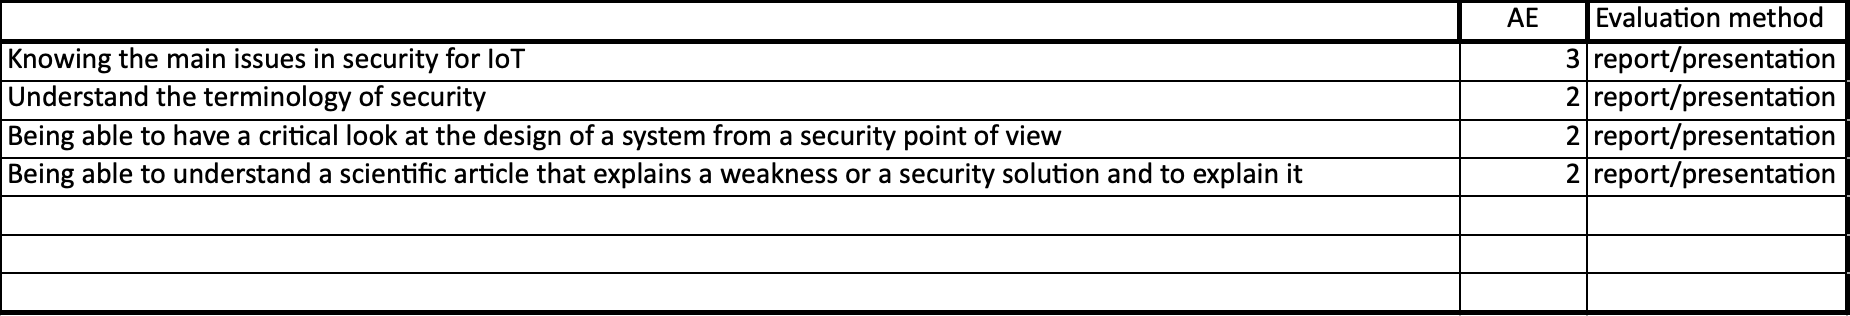
\includegraphics[width=0.8\textwidth]{image/Security.png}
    \caption{Security Unit}
    \label{fig:Security}
\end{figure}


\subsection{apprenticeship}

\subsubsection{Descriptive}
\chapter{Communication unit}
\thispagestyle{fancy}


\section{Energy For Connected Oject}

\subsection{Overview of the Energy for Connected Objects Course}

As part of the Innovative Smart System specialization in the 5th year, the course titled Energy for Connected Objects focuses on energy solutions for connected objects (IoT), addressing innovative techniques such as ambient energy harvesting and wireless energy transfer. The objective of this course is to provide students with an in-depth understanding of modern methods for managing and generating energy for connected objects. These systems are crucial in a context where energy autonomy and sustainability are essential for the development of the Internet of Things.

The course is structured with a combination of lectures and practical work. The four theoretical sessions cover topics ranging from electricity generation and storage to ambient energy harvesting techniques (such as light, vibrations, and electromagnetic fields) and advanced wireless energy transfer methods (including near-field and far-field electromagnetic solutions). These concepts help to understand how to power connected objects wirelessly and without batteries, by exploiting available energy sources in the environment.

The two practical sessions allow students to apply these concepts by designing an emulator for connected objects and characterizing an electromagnetic energy harvesting system. Evaluation is based on a group lab report and an in-depth study of energy autonomy options for an innovative project. This study includes exploring battery-free power supply possibilities, paving the way for sustainable IoT projects. Additionally, the course provides a series of academic resources to further knowledge in energy harvesting and wireless transfer, which are essential for developing efficient and environmentally responsible IoT devices.


\subsection{Technical Foundations of Energy-Autonomous IoT Systems}

The technical dimension of this course focuses on two key areas: ambient energy harvesting and wireless energy transfer, with particular attention to practical aspects and technical challenges in designing energy-autonomous IoT systems.

Ambient Energy Harvesting
This technique involves capturing energy from the environment and converting it into electricity to power connected objects. Ambient energy sources include:

\begin{itemize}
    \item Light: primarily through photovoltaic cells that capture both solar and artificial light.
    \item Mechanical (kinetic): using electromagnetic, piezoelectric, or electrostatic transducers capable of converting vibrations or motion into electrical energy.
    \item Thermal: using thermal transducers like thermoelectric devices, which generate electricity from temperature gradients.
    \item Electromagnetic: using capacitive and inductive transducers to capture ambient electromagnetic fields.
\end{itemize}


This approach allows for continuous power, although it depends on the proximity of field sources. Each type of energy harvesting presents challenges related to availability, stability, and energy efficiency. Optimization techniques such as using hybrid transducers or transducer networks (series/parallel topologies) can improve the efficiency of energy collection for low-power IoT devices.

Wireless Energy Transfer
This field covers methods that enable the transmission of energy without cables, focusing on powering connected objects via dedicated energy sources, which are often more reliable and predictable than ambient sources. The main wireless energy transfer techniques include:

\begin{itemize}
\item Optical (light): using lasers or infrared for long-distance transfers, requiring a direct line of sight.
\item Acoustic: using ultrasound, especially for specific applications and short-range transfer.
\item Electromagnetic: which is divided into near-field transfer (capacitive or inductive coupling, suitable for short distances with high efficiency) and far-field transfer (radio or microwave waves), enabling longer ranges but typically with lower efficiency.
\end{itemize}


To maximize the energy efficiency of these wireless systems, devices like rectennas (rectifying antennas) are used, converting RF waves into DC current. Optimal rectenna design involves selecting an appropriate frequency, using impedance matching circuits, and carefully configuring the rectifier to minimize losses. Signal modulation techniques, impedance management, and waveform optimization are essential to reduce energy dissipation and meet the power and autonomy requirements of connected objects.

This course provides a technical understanding of energy management solutions for autonomous IoT systems, covering the design of autonomous sensors, reducing energy consumption, and best practices to optimize the efficiency of energy harvesting and transfer devices. These skills are crucial in the development of sustainable IoT applications, ranging from smart homes to industrial sensor networks.


\subsection{Reflections and Applications of Wireless Energy Transmission}

The Energy for Connected Objects course was highly enriching, even though the foundational knowledge was already familiar to most students. The real value lay in connecting various building blocks of knowledge in a coherent and practical way.

Prior to this course, I had never implemented wireless energy transmission in either my personal or professional life. Thanks to the lectures and hands-on practical sessions, I now feel confident in designing and implementing such systems. The practical exercises were well-aligned with the course content and enabled me to achieve my first successful wireless energy transmission.

While I do not currently plan to work in this specific field, as my professional interests lean more toward software development in the aerospace sector, I can already envision potential applications for this technology. For example, wireless energy transmission could be used within satellites to reduce weight by eliminating cables. However, further research would be needed to determine if this approach is viable in the vacuum of space.

This course provided valuable general knowledge that could be applied to personal projects and opened new opportunities for my future job search.

I will now proceed to self-assess my performance on the key aspects of this course :

\begin{itemize}
    \item Mastering the architectures of an energy management system, simple storage, energy recovery, know of to size the storage capacity: 4
    \item understand and Master optimization of Communication protocols for IoT with respect to energy limitations: 4
\end{itemize}


\section{Wireless Sensor Network}

\subsection{Course Structure: Theory, Research, and Practical Work}

The course Towards Internet of Things (IoT) and Wireless Sensor Networks (WSN), led by Professor Daniela Dragomirescu, aims to equip students with the necessary skills to design, implement, and deploy wireless sensor and actuator networks. These networks are critical to the development of IoT systems, focusing on aspects such as energy efficiency, robustness, and ease of deployment.

Wireless communication technologies, including GSM, GPRS, EDGE, and UMTS, have paved the way for the emergence of IoT and related systems like WSN, Ambient Intelligence, and Cyber-Physical Systems. This course explores the architectural and operational principles of IoT and WSN, emphasizing:

\begin{itemize}
    \item Designing energy-efficient systems.
    \item Developing protocols for enhanced reliability, synchronization, and localization
    \item Exploring the challenges of real-world deployment, including battery constraints and security.
\end{itemize}

The course combines theoretical lectures with practical assignments:

\begin{itemize}
    \item Theoretical Lectures: Cover IoT architecture, challenges in WSN, and cross-layer optimization.
    \item Research Work : Students worked on group and individual projects analyzing various protocols, such as LoRa, Sigfox, ZigBee, and BLE. Tasks included examining physical and MAC layers, energy consumption, and specific use cases.
    \item A pratical work to define the specification and a simulation of hand made MAC protocols with physical layer.
\end{itemize}

This course bridges academic learning with practical applications, highlighting use cases in fields such as aeronautics, healthcare, and smart infrastructure. It offers insights into the real-world challenges and opportunities presented by IoT technologies, preparing students for diverse professional paths.

\subsection{Energy-Efficient Strategies in Wireless Sensor Networks}

The IoT ecosystem integrates sensing, data collection, analysis, and actionable insights. A typical IoT architecture involves:

\begin{itemize}
    \item Sensors and Actuators: Gather physical data and initiate actions.
    \item Wireless Communication: Ensures seamless data transfer.
    \item Internet Connectivity: Enables remote monitoring and control.
    \item Data Analysis: Derives meaningful insights from collected data.
\end{itemize}

Wireless Sensor Networks play a pivotal role in this architecture, addressing challenges like energy autonomy, synchronization, and data routing.
ne of the major challenges in deploying WSNs is the reliance on batteries. The course introduces energy-harvesting techniques such as solar and thermal harvesting.
The main objective witt the energy is to made a energy-efficient erotocols with MAC and routing layers designed to minimize power consumption.

The course delves deeply into protocols optimized for WSN, emphasizing their MAC and physical layers. Key considerations include:

\begin{itemize}
    \item Synchronization: Ensures data consistency and reduces latency.
    \item Localization: Provides spatial awareness for sensor nodes.
    \item Security: Implements measures to safeguard data integrity..
\end{itemize}

Protocols like ZigBee and BLE were analyzed in assignments for their trade-offs in power consumption, range, and data rates, providing insights into their suitability for different applications.
Our groupe has to made research about BLE, you can find our work in the annexe part.

The second assement made a focus on MAC protocols, during our research we gain a better understanding of different type of access: 
explores several MAC protocols designed for wireless sensor networks (WSN) and the Internet of Things (IoT). Traditional approaches such as FDMA, TDMA, and CDMA divide resources by frequency, time, or codes. While straightforward, they face limitations in synchronization and energy efficiency. 
Contention-based protocols like CSMA/CA, S-MAC, and T-MAC use mechanisms to avoid collisions, with improvements such as programmed sleep cycles to conserve energy. Energy-optimized protocols, including B-MAC and L-MAC, focus on managing active and passive periods to reduce consumption but are less suited for mobile environments. 
Advanced protocols like GAF incorporate location-based management, dividing the network into cells to activate only necessary nodes, optimizing energy while supporting mobility. Each protocol addresses specific needs, from energy stability to flexibility for dynamic IoT applications.


\subsection{Reflections on the Impact of the WSN Course}

The WSN (Wireless Sensor Networks) course was one of the most impactful courses of the year for me. It stood out as one of the classes that introduced the most new information and concepts. The workload for this course was notably higher compared to others, largely due to the novelty of the material. However, I found it invaluable, as it significantly enhanced my understanding of the processes involved in information transfer.

This course was particularly important because it served as a central pillar for the year, especially within the communication module. The knowledge gained here was directly applied in other courses, such as those on 3G to 6G technologies and energy systems. It also played a key role in the Innovative Project, which was multidisciplinary in nature and required a synthesis of skills and knowledge from various domains.

The assignments and deliverables were especially critical, and active participation during lectures was essential for grasping and applying the course concepts effectively.

Although I have not yet had the opportunity to apply the knowledge gained in a professional setting due to the software-focused nature of my apprenticeship I recognize the immense potential of WSN protocols. While I plan to continue in the software field, I believe exploring WSN applications after my studies could open up exciting opportunities given the vast range of possibilities these technologies offer.

I will now proceed with my self-assessment.

\begin{itemize}
    \item Be able to analyse and evaluate optimal wireless network technologies: 4
    \item Be able to suggest optimal technological solutions for IoT networks: 3
    \item Know the main processing techniques used for digital communication and know how to explain the basic Structure of digital: 4
    \item Understand and master optimisation of communication protocols with respect to security concerns: 3
\end{itemize}


\section{5G technologies}

\subsection{Evolution of Mobile Networks: From 3G to 6G}

The course titled "From 3G to 6G," taught by Professor Étienne Sicard at INSA Toulouse, delves into the evolution of mobile technologies, from their inception to the cutting-edge advancements shaping the future. Aimed at fifth-year students, this course provides a comprehensive understanding of the technical, economic, and environmental aspects of mobile networks. It highlights the major technological transitions that have defined each generation and explores innovations paving the way toward the 6G era.

The course covers several key themes. The first section focuses on the miniaturization of electronic components, discussing advances in transistor design, including the shift from traditional MOSFETs to modern architectures like FinFETs and Nano-Sheet FETs. This evolution is framed within the broader context of the global transformation of the electronics industry and its impact on mobile network performance.

The second section revisits the history of mobile generations, from 3G to 6G, emphasizing key technological milestones and applications associated with each era. The 3G era, marked by the introduction of UMTS, was pivotal in enabling mobile data services. Subsequently, 4G introduced LTE, revolutionizing multimedia applications by providing significantly higher bandwidth. The 5G era brought the integration of the Internet of Things (IoT) and the utilization of millimeter-wave frequency bands, dramatically enhancing network capacity and speed.

Lastly, the course reflects on emerging technologies and the future of telecommunications, particularly through the roadmaps toward 6G outlined by industry leaders like Nokia, Huawei, and Orange. These roadmaps introduce transformative innovations such as Zero-Energy Devices and cyber-physical systems, which are poised to redefine connectivity.

A critical part of the course involved group presentations. Our group chose to focus on the topic of Starlink, an innovative satellite internet system by SpaceX. This project was pivotal in contextualizing the theoretical knowledge gained during the course, linking it with real-world applications.
\subsection{Scientific Foundations and Innovations in Mobile Telecommunications}

The technical aspect of the course immerses students in the scientific foundations and innovations underpinning mobile telecommunications. A major focus is on technological miniaturization, which has revolutionized electronic device design over the years. With the continuous reduction in transistor size, evolving from traditional MOSFETs to FinFETs and Nano-Sheet FETs, the performance of electronic chips has greatly improved. These advances have enabled the production of more compact and energy-efficient devices capable of handling increasingly large volumes of data.

The course also explores the evolution of mobile generations, shedding light on the bandwidth requirements and modulation technologies specific to each generation. The 3G era marked the advent of mobile internet with UMTS, while 4G, through LTE, revolutionized the use of multimedia applications with higher data speeds. The 5G era introduced millimeter-wave frequencies (26 GHz) and advanced technologies such as massive MIMO and beamforming, paving the way for sophisticated applications like autonomous vehicles and connected healthcare. Looking ahead, 6G, anticipated by 2030, aims to exploit even higher frequencies, exceeding 100 GHz, enabling ultra-fast data rates and minimal latency. However, these advancements come with significant technical challenges, including signal attenuation at high frequencies and increased energy consumption.

The exploration of ultra-high frequencies (UHF and beyond) is a central theme of the course. While 5G primarily operates between 3.4 GHz and 26 GHz, 6G aims to expand into frequencies exceeding 100 GHz, encompassing the W and D bands (130–174 GHz). This transition toward higher frequencies unlocks unique opportunities for applications such as augmented reality, telemedicine, and global connectivity via satellite constellations. However, it also introduces challenges related to wave propagation and the need for more efficient antenna designs.

Our group presentation on Starlink tied into the technical elements of the course by examining its use of low Earth orbit (LEO) satellites operating at frequencies between 10.7 GHz and 12.7 GHz. We analyzed the implications of satellite constellations for global connectivity and their technical challenges, such as frequency interference and latency. Additionally, we highlighted the role of innovative technologies in overcoming deployment hurdles and meeting the increasing demands for broadband access. This project served as a practical extension of the course’s technical content, allowing us to apply theoretical knowledge to a real-world case study.

\subsection{Reflections on the Course and Professional Insights}


I perceived this course as a valuable addition to my general knowledge, as it did not present significant challenges in terms of comprehension. Delving deeper into the history of mobile technologies provided me with a clearer understanding of the future implications of this field, along with the technical challenges it poses for the environment and end users.

One of the standout aspects of this course was the freedom and variety of topics available for presentations. This flexibility allowed us to conduct research on subjects we were passionate about, making the work both engaging and enjoyable. Personally, I greatly appreciated this approach, as it encouraged active participation and made the learning experience more meaningful.

From a professional perspective, I have already had opportunities to explore and gain insights into the mobile technology sector. However, my focus has primarily been on GNSS (Global Navigation Satellite Systems) technologies. While the mobile technology field is a rapidly growing industry with promising career opportunities, I currently do not envision it as my primary career path. Nevertheless, the knowledge and insights gained from this course remain highly relevant and valuable for my broader professional development

I will now proceed with my self-assessment.

\begin{itemize}
    \item Understand the major development phases for mobile communications and development of the associated technology: 4
    \item Understand the impact of new technology: 4
\end{itemize}

\section{Emerging Network}
\subsection{Descriptive}
\subsection{Technical}
\subsection{Analytic}


\section{Communication protocols for LP-WPAN}
\subsection{Descriptive}
\subsection{Technical}
\subsection{Analytic}

\section{Embedded IA for IoT}
\subsection{Descriptive}
\subsection{Technical}
\subsection{Analytic}


\chapter{Middleware and service}

\section{Cloud and Edge Computing}
\subsection{Descriptive}


The Cloud and Edge Computing course, taught by Dr. Sami YANGUI, explores key concepts and technologies related to distributed computing, cloud computing, and edge computing. This course is essential for students specializing in Innovative Smart Systems, as it covers the fundamentals needed to understand how Internet of Things (IoT) systems interact with cloud and edge architectures, thus optimizing data processing and management.

Key concepts include:

Distributed Computing: This approach uses multiple interconnected components to work together in a single environment, with coordinated actions to achieve common goals. These systems help optimize communication and resource sharing within IoT applications.

Cloud Computing: This model relies on access to a vast pool of virtualized resources, available on demand, with a "pay-as-you-go" billing model. The cloud offers great flexibility for IoT infrastructure and applications, reducing operational costs.

Edge Computing: This technique brings data processing closer to the sources, reducing latency and enabling real-time processing. Edge computing is especially relevant for IoT applications requiring high responsiveness, such as predictive maintenance, fleet management, or autonomous navigation systems.

The course also covers virtualization and the role of hypervisors in enabling the simultaneous operation of multiple operating systems on a single physical infrastructure, which is crucial for resource management in cloud and edge environments.

\subsection{Technical}

Technically, the course delves into the architectures needed to set up cloud and edge systems suitable for the constraints of IoT applications. The concept of virtualization is central, particularly with the use of type-1 (bare-metal) and type-2 (hosted) hypervisors, which allow for flexible and efficient resource allocation. These hypervisors also ensure process isolation, reducing the risk of conflicts and optimizing security.

One key technical aspect of the course is cloud federation and the portability of applications between different environments. Through federation, multiple cloud services can collaborate to better manage load spikes. For example, in fleet management applications, a hybrid cloud infrastructure can dynamically distribute tasks between the centralized cloud and edge nodes to ensure continuous availability and low latency.

The practical work allows students to deepen their use of containers (such as with Docker) and cluster management via Kubernetes. As part of the lab project, students set up a hybrid cloud-edge architecture capable of handling the mobility and dynamic availability of edge nodes, simulating events like road accidents or construction sites. The goal is to maintain reliable service throughout a journey by replicating services across the network and migrating services between nodes when necessary.

Finally, the course covers deployment models, such as IaaS (Infrastructure as a Service), PaaS (Platform as a Service), and SaaS (Software as a Service), which offer varying levels of control and flexibility. Students learn to choose the appropriate model based on the specific needs of IoT applications, as well as how to design scalable and autonomous services to optimize costs and performance.

\section{Analytical Part}
Voici le contenu de la première section.




% Inclusion des chapter

\section{Annexes}

\includepdf[scale=0.7,pages={1 21}]{annexe/BIENDOU-BRUNETTO-VASSEUR-Cloud_Computing_Report.pdf}



\end{document}
